%%%%%%%%%%%%%%%%%%%%%%%%%%%%%%%%%%%%%%%%%%%%%%%%%%%%%%%%%%%%%%%%%%%%%
% Template de Artigo
% XXIX ENMC – Encontro Nacional de Modelagem Computacional
% XVII ECTM – Encontro de Ciência e Tecnologia de Materiais
%%%%%%%%%%%%%%%%%%%%%%%%%%%%%%%%%%%%%%%%%%%%%%%%%%%%%%%%%%%%%%%%%%%%%

\documentclass[12pt,fleqn]{article}

%%%%%%%%%%%%%%%%%%%%%%%%%%%%%%%%%%%%%%%%%%%%%%%%%%%%%%%%%%%%%%%%%%%%%
% CONFIGURAÇÃO DE IDIOMA E CODIFICAÇÃO
%%%%%%%%%%%%%%%%%%%%%%%%%%%%%%%%%%%%%%%%%%%%%%%%%%%%%%%%%%%%%%%%%%%%%

\usepackage[utf8]{inputenc}   % Codificação UTF-8
\usepackage[T1]{fontenc}      % Codificação de fontes
\usepackage[brazil]{babel}    % Português do Brasil (Babel moderno)

%%%%%%%%%%%%%%%%%%%%%%%%%%%%%%%%%%%%%%%%%%%%%%%%%%%%%%%%%%%%%%%%%%%%%
% PACOTES DO TEMPLATE
%%%%%%%%%%%%%%%%%%%%%%%%%%%%%%%%%%%%%%%%%%%%%%%%%%%%%%%%%%%%%%%%%%%%%

\usepackage{setup/config}     % Arquivo de estilo do evento
\usepackage{natbib}           % Sistema de citações
\usepackage{graphicx}         % Inserção de figuras
\usepackage{color}            % Controle de cores
\usepackage{wallpaper}        % Imagens de fundo
\usepackage{hyperref}         % Links e referências
\usepackage{titlesec}         % Controle de títulos
\usepackage{float}            % Permite usar [H] em figuras/tabelas
\usepackage{fancyhdr}         % Cabeçalhos e rodapés

%%%%%%%%%%%%%%%%%%%%%%%%%%%%%%%%%%%%%%%%%%%%%%%%%%%%%%%%%%%%%%%%%%%%%
% DIRETÓRIO DAS FIGURAS
%%%%%%%%%%%%%%%%%%%%%%%%%%%%%%%%%%%%%%%%%%%%%%%%%%%%%%%%%%%%%%%%%%%%%

\graphicspath{{figures/}}

%%%%%%%%%%%%%%%%%%%%%%%%%%%%%%%%%%%%%%%%%%%%%%%%%%%%%%%%%%%%%%%%%%%%%
% AJUSTE DE ESPAÇAMENTO NA BIBLIOGRAFIA
%%%%%%%%%%%%%%%%%%%%%%%%%%%%%%%%%%%%%%%%%%%%%%%%%%%%%%%%%%%%%%%%%%%%%

% Reduz espaçamento entre referências
\let\OLDthebibliography\thebibliography
\renewcommand\thebibliography[1]{%
\OLDthebibliography{#1}
\setlength{\parskip}{0pt}
\setlength{\itemsep}{0pt plus 0.3ex}
}

%%%%%%%%%%%%%%%%%%%%%%%%%%%%%%%%%%%%%%%%%%%%%%%%%%%%%%%%%%%%%%%%%%%%%
% TÍTULO DO ARTIGO
%%%%%%%%%%%%%%%%%%%%%%%%%%%%%%%%%%%%%%%%%%%%%%%%%%%%%%%%%%%%%%%%%%%%%

\title{INSTRUCTIONS FOR PREPARATION AND SUBMISSION OF PAPERS FOR PUBLICATION IN THE PROCEEDINGS OF XXIX ENMC / XVII ECTM}

%%%%%%%%%%%%%%%%%%%%%%%%%%%%%%%%%%%%%%%%%%%%%%%%%%%%%%%%%%%%%%%%%%%%%
% AUTORES E AFILIAÇÕES
%%%%%%%%%%%%%%%%%%%%%%%%%%%%%%%%%%%%%%%%%%%%%%%%%%%%%%%%%%%%%%%%%%%%%

\author{
\rm
\begin{tabular}{l}
\textbf{First Author}$^{1}$ - {\textnormal e-mail}\\
\textbf{Second Author}$^{2}$ - {\textnormal e-mail}\\
\textbf{Third Author}$^{3}$ - {\textnormal e-mail}\\
{\fontsize{11}{0}\selectfont $^{1}$Universidade Federal do Rio Grande – Rio Grande – RS}\\
{\fontsize{11}{0}\selectfont $^{2}$Universidade Federal do Rio Grande – Santo Antônio da Patrulha – RS}\\
{\fontsize{11}{0}\selectfont $^{3}$Universidade Federal do Rio Grande – São Lourenço do Sul – RS}
\end{tabular}
}

%%%%%%%%%%%%%%%%%%%%%%%%%%%%%%%%%%%%%%%%%%%%%%%%%%%%%%%%%%%%%%%%%%%%%
% RODAPÉ ESPECIAL DA PRIMEIRA PÁGINA
%%%%%%%%%%%%%%%%%%%%%%%%%%%%%%%%%%%%%%%%%%%%%%%%%%%%%%%%%%%%%%%%%%%%%

\fancypagestyle{firstpagestyle}
{
\renewcommand{\headrulewidth}{0pt}

\fancyfoot[C]{
\footnotesize
\parbox{15cm}{
\centering
\fontsize{7.5}{0}\selectfont\it
XXIX ENMC – Encontro Nacional de Modelagem Computacional\\
XVII ECTM – Encontro de Ciência e Tecnologia de Materiais\\
06 a 09 de outubro de 2026 - Bento Gonçalves - RS
}}
}

%%%%%%%%%%%%%%%%%%%%%%%%%%%%%%%%%%%%%%%%%%%%%%%%%%%%%%%%%%%%%%%%%%%%%
% INÍCIO DO DOCUMENTO
%%%%%%%%%%%%%%%%%%%%%%%%%%%%%%%%%%%%%%%%%%%%%%%%%%%%%%%%%%%%%%%%%%%%%

\begin{document}

\pretolerance=10000

%%%%%%%%%%%%%%%%%%%%%%%%%%%%%%%%%%%%%%%%%%%%%%%%%%%%%%%%%%%%%%%%%%%%%
% LOGO DO EVENTO
%%%%%%%%%%%%%%%%%%%%%%%%%%%%%%%%%%%%%%%%%%%%%%%%%%%%%%%%%%%%%%%%%%%%%

\begin{figure}
\centering

\includegraphics[width=6.25in]{logo.png}
\end{figure}

\vspace{-3cm}

%%%%%%%%%%%%%%%%%%%%%%%%%%%%%%%%%%%%%%%%%%%%%%%%%%%%%%%%%%%%%%%%%%%%%
% TÍTULO
%%%%%%%%%%%%%%%%%%%%%%%%%%%%%%%%%%%%%%%%%%%%%%%%%%%%%%%%%%%%%%%%%%%%%

\maketitle

\pagestyle{empty}
\thispagestyle{firstpagestyle}

%%%%%%%%%%%%%%%%%%%%%%%%%%%%%%%%%%%%%%%%%%%%%%%%%%%%%%%%%%%%%%%%%%%%%
% RESUMO
%%%%%%%%%%%%%%%%%%%%%%%%%%%%%%%%%%%%%%%%%%%%%%%%%%%%%%%%%%%%%%%%%%%%%

\begin{abstract}
This document-template provides detailed instructions for preparing and submitting a paper to XXIX ENMC – National Meeting on Computational Modeling / XVII ECTM – Meeting on Materials Science and Technology. Please follow these instructions: a) type the body of the paper in a single column; b) use 5 to 10 A4-size pages (21 cm $\times$ 29.7 cm), each formatted with 2.5 cm margins on all sides except at the top of the page (do not print any border around the text and do not insert page numbers); c) use 12 pt Times New Roman throughout, except on affiliation identification; d) type up to 200 words in the abstract, in italics; e) always use single-spaced lines, justified alignment; f) cite references by last name (year) and list in alphabetical order by author last name at the end; g) supply good quality figures/photographs being recommended a resolution of 300 dpi (color figures can be used); h) define all symbols as they appear in the text; i) use only SI units. The paper may be written in English, Portuguese or Spanish.
\end{abstract}

\keywords{\em{First keyword, Second keyword, Third keyword (up to 5 keywords)}}

%%%%%%%%%%%%%%%%%%%%%%%%%%%%%%%%%%%%%%%%%%%%%%%%%%%%%%%%%%%%%%%%%%%%%
% CABEÇALHO DAS DEMAIS PÁGINAS
%%%%%%%%%%%%%%%%%%%%%%%%%%%%%%%%%%%%%%%%%%%%%%%%%%%%%%%%%%%%%%%%%%%%%

\fancyhead[L]{\footnotesize{\fontsize{7.5}{0}\selectfont\it
XXIX ENMC, XVII ECTM\\
06 a 09 de outubro de 2026}}

\renewcommand{\headrulewidth}{0pt}

\fancyfoot[C]{
\footnotesize
\parbox{15cm}{
\centering
\fontsize{7.5}{0}\selectfont\it
XXIX ENMC – Encontro Nacional de Modelagem Computacional\\
XVII ECTM – Encontro de Ciência e Tecnologia de Materiais\\
06 a 09 de outubro de 2026 - Bento Gonçalves - RS
}}

\rhead{}

\pagestyle{fancy}

%%%%%%%%%%%%%%%%%%%%%%%%%%%%%%%%%%%%%%%%%%%%%%%%%%%%%%%%%%%%%%%%%%%%%
% INÍCIO DO TEXTO
%%%%%%%%%%%%%%%%%%%%%%%%%%%%%%%%%%%%%%%%%%%%%%%%%%%%%%%%%%%%%%%%%%%%%

\section{INTRODUCTION [Times New Roman 12pt, all capital letters, bold]}

The paper should generally follow the structure Introduction, Methodology, Results and Discussion, Conclusions and References as described in the typing instructions. The Proceedings of XXIX ENMC / XVII ECTM, which include the full versions of all papers to be presented at the meeting, will be published in digital media. Therefore, it is extremely important that you prepare the PDF digital version of your contribution in accordance with the present instructions. The file size must be less than 4 MB.

The Editorial Committee will evaluate all submitted papers.

\subsection{Alterations}

Hyperref package inclusion; Eq.~(\ref{eq1}) or Fig.~\ref{fig1}

Bibliography with apalike, through .bib file

For references, use cite for external or direct citacion ``In \cite{delvecchio1992}...'', and citep for in parenthesis/indirect \citep{delvecchio1992}.

Examples inside .bib for conference~\citep{davies2008}, for book~\citep{horrocks2016}, for in-collection~\citep{linganiso2016}, for article~\citep{abhari2017}, for PhD thesis~\citep{delvecchio1992}, and for manual/standard~\cite{iso2060}.



\section{TYPING INSTRUCTIONS}
The paper must be written in English, Portuguese or Spanish. If written in Portuguese or Spanish, a translation of title, abstract and keywords into English must be provided at the end of the paper (after the reference list).
% \ \ \ \
%\newpage %

\subsection{Paper length}
The full paper including figures and tables must have at least 5 pages, but is limited to 10 A4-size pages (21 cm x 29.7 cm). Please limit your paper by writing concisely, rather than by reducing figures or tables to a size at which symbols/labels become difficult to read.

\subsection{Page format}
Each A4-size page should be formatted with 2.5 cm margins on all sides, except at the top. This defines the printable area. Inside this area, the text must be arranged in a single column. Please do not print any border around the text and do not insert page numbers.

The final paper should look like this document.

\subsection{General text specifications}

The paper must be typed using 12 pt Times New Roman throughout the text, as in the present document. This includes title, headings, and figure and table captions.

\vspace{0.5cm} % Example spaces

\textbf{\textit{Paper title.}} The title should be in boldface type, all capital letters and centered on the page and must not exceed three lines. It should be single spaced if longer than one line. Skip one line (12 pt) between the title and the first author.

\vspace{0.5cm} % Example spaces

\textbf{\textit{Author(s) and affiliation.}} Type authors names in boldface type, flush left, one per line, including first name, middle and last name, followed by the e-mail address (not boldfaced). After the name put in superscript the number, related to the affiliation. The authors names should be followed by the corresponding affiliation, which should be in regular type (neither boldfaced nor italicized). After presenting affiliations should skip two lines (24 pt) between the last affiliation and the abstract.

\vspace{0.5cm} % Example spaces

\textbf{\textit{Abstract and keywords.}} Type the heading \textbf{\textit{Abstract.}} in boldface italics, flush left, followed by a period. On the same line, type the abstract in italics, justified alignment. The abstract should be no longer than 200 words. Skip one line, then type the heading \textbf{\textit{Keywords:}} (don't forget the colon) in boldface italics, flush left and type 3 to 5 keywords, separated by commas, with only the first letter of each keyword capitalized. Skip two lines (24 pt) between the keywords and the body of text.

\vspace{0.5cm} % Example spaces

\textbf{\textit{Headings.}} Type a first-level head (section) in all capital letters, boldface type, flush left. Begin by typing the Arabic number followed by a period, then type the head title 0.75 cm (or 7 blank spaces) from the left margin. Leave one blank line above and one below this head.

For a second-level head (subsection), capitalize only the first letter, using boldface type, flush left. Begin by typing the double number, then type the sub-head title 0.75 cm from the left margin. Leave one blank line above and one below this head.

Do not number third-level heads (sub-subsection). Use boldface italics, capitalizing only the first letter and indenting 0.75 cm from the left margin. Follow it by a period and start the text immediately. Leave one blank line above this head.

\vspace{0.5cm} % Example spaces
%
\textbf{\textit{Body of text.}} The text should be typed using single-spaced lines and justified alignment. Start each paragraph 0.75 cm from the left margin and allow no space between paragraphs.

\subsection{Structure of the paper}

The document should follow the conventional structure of scientific papers. Although variations may occur depending on the nature of the research, the recommended organization includes the following sections:

\textbf{Introduction.} This section should present the context of the study, the research problem, the objectives of the work and the relevant background from the literature.

\textbf{Methodology.} This section should describe the methods, models, experimental procedures, datasets or computational approaches used in the research, allowing the work to be understood and, when possible, reproduced.

\textbf{Results and Discussion.} This section should present the results obtained in the study and discuss their significance, comparing them with related work whenever appropriate.

\textbf{Conclusions.} This section should summarize the main findings of the work and highlight the contributions of the research.

\textbf{References.} All works cited in the manuscript must be listed at the end of the document. The references must be managed using BibTeX and formatted according to the \texttt{apalike} bibliography style. Only works cited in the text using commands such as \verb|\cite{}| will appear in the reference list.

Additional sections may be included when necessary (e.g., theoretical background, case study, acknowledgements or appendix), provided that the overall organization of the manuscript remains clear and coherent.



\subsection{Equations, symbols and units}
Indent an equation 1 cm (or 10 spaces) from the left margin. Number it with an Arabic number enclosed in parentheses, placed flush right. Allow one blank line above and one below each equation. For example:
\begin{equation}
\vec{q}_{r}=-4\pi r^{2}k\frac{dT}{dr}
\label{eq1}
\end{equation}
%%%here space

When referring to an equation in the text write Eq.(\ref{eq1}), except at the beginning of a sentence, where Equation (\ref{eq1}) should be used.

Symbols should be italicized throughout the text. Define all symbols as they appear in the text. A nomenclature section is not necessary.

All data, including those shown in tables and figures, must be reported in SI units.

\subsection{Figures and tables}
Figures and tables should be inserted as close as possible to their mention in the text. Enclosed text and symbols must be clearly readable; avoid small symbols. Supply good quality pictures and illustrations.

Figures and tables and their captions should be centered in the text. Place figure caption below the figure, leaving one blank line between them. Place table title above the table, also leaving one blank line between them. Leave one blank line between the table or figure and the adjacent text. Color figures can be used.

Number figures and tables consecutively using Arabic numerals (e.g., Figure 1, Figure 2, Table 1, Table 2). Refer to them in the text as Table \ref{table1} and Fig. \ref{fig1} (except at the beginning of a sentence, where Figure \ref{fig1}  should be used).


% TABLE EXAMPLE
\begin{table}[H] % !htbp
\caption{Input parameters}

\centering{}
\begin{tabular*}{\textwidth}{@{\extracolsep{\fill}}ccc|cc}        % {0.8\textwidth}
\hline
Method LJ & Configuration && Method R2W & Configuration\tabularnewline
\hline
$k_1$ (W/mK)  & $[0,0; 0,1]$ && $k_1$ (W/mK) & $[0, 0; 0,1]$\tabularnewline
\hline
$k_2$ (W/mK) & $[0,0; 0,1]$ && $k_2$ (W/mK) & $[0, 0; 0,1]$\tabularnewline
\hline
$n$ & $1,0$ && $n$ & $1,0$\tabularnewline
\hline
\end{tabular*}
{\footnotesize\centering Fonte: Autor (2026)\par}
\label{table1}
\end{table}

\begin{figure}[!htbp] %h or !htbp
\vspace{-2pt}
\begin{center}
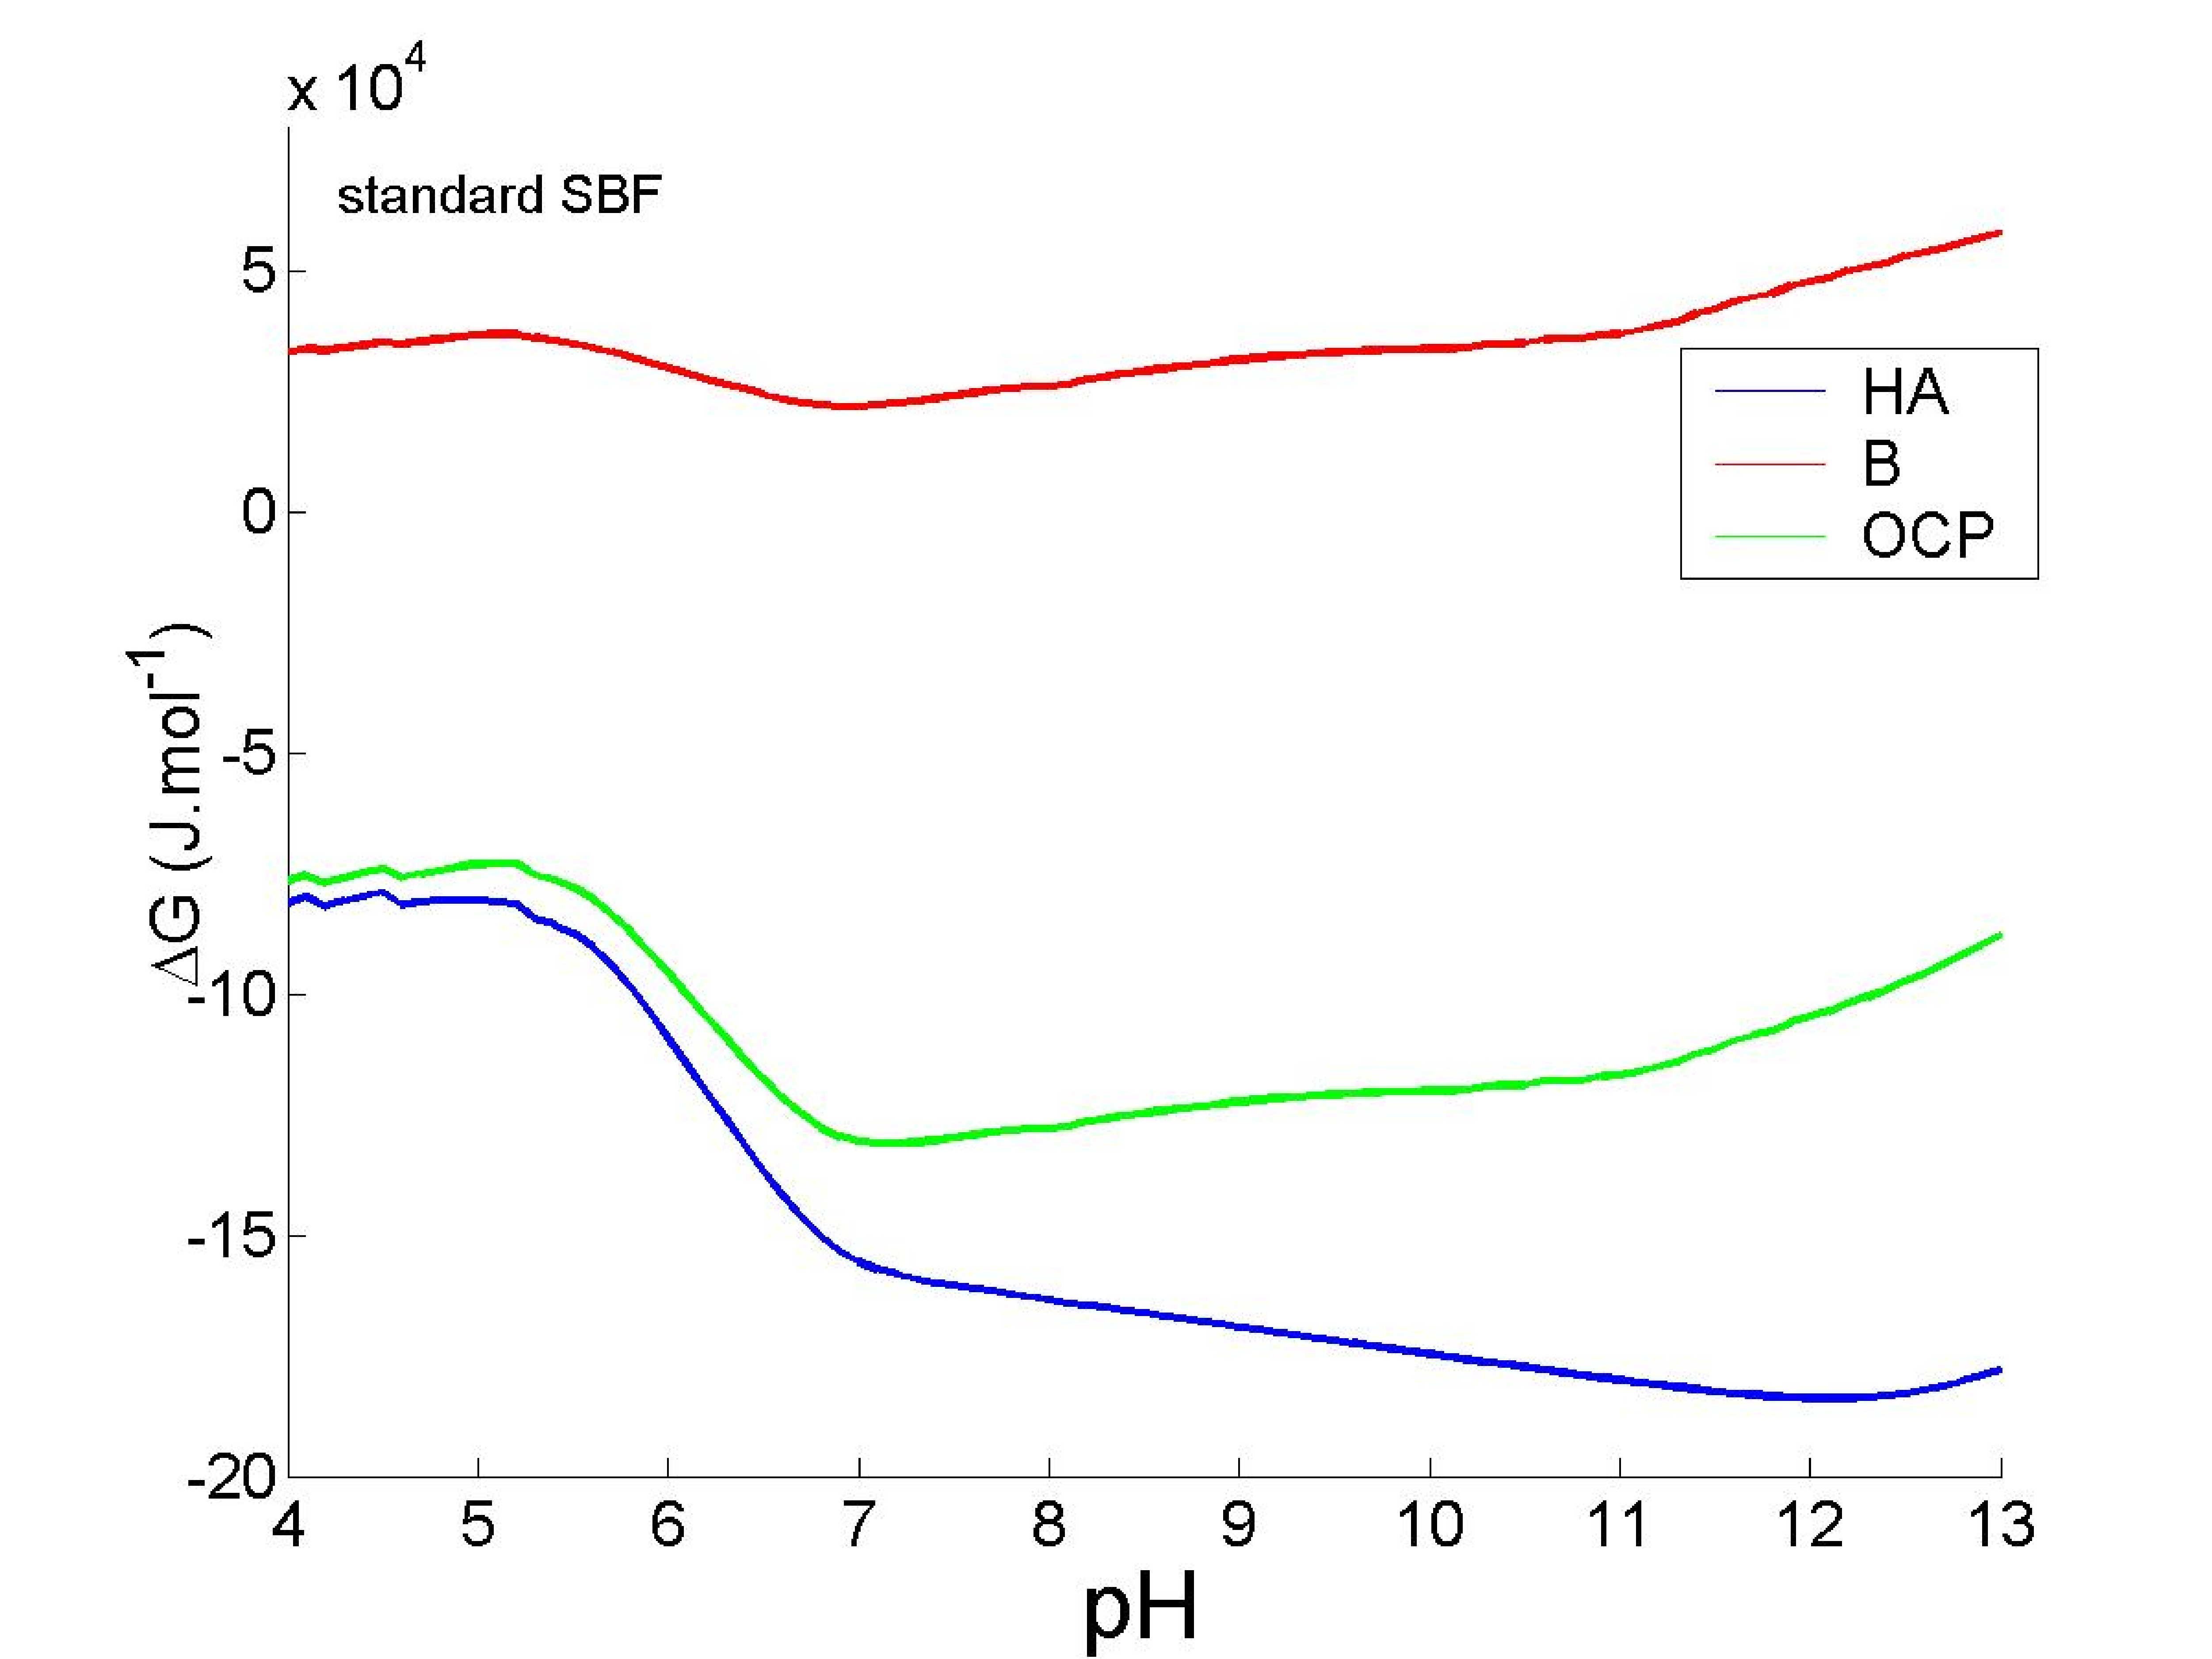
\includegraphics[height=6.7cm,width=9cm]{figura_1.png}%
\caption{Gibbs free energy variations: simulated results.}
{\footnotesize\centering Fonte: Autor (2026)\par}
\label{fig1}%
\end{center}
\end{figure}

Label coordinates in plots and add the corresponding units. Similarly, label columns/rows in tables and add the units.

\subsection{Permission}
You are responsible for making sure that you have the right to publish everything in your paper. If you use material from a copyrighted source, you may need to obtain permission from the copyright holder.

\subsection{Use of Generative Artificial Intelligence Tools}

Authors must disclose the use of Generative Artificial Intelligence (AI) tools in the preparation of the manuscript. According to research integrity guidelines the use of Generative AI tools must be explicitly declared whenever they are employed at any stage of the research or manuscript preparation, including conception, data analysis, text writing, editing or translation.

When such tools are used, authors must clearly indicate the name of the tool and its purpose in the manuscript, preferably in the Acknowledgements section or in a dedicated statement. Authors remain fully responsible for the accuracy, originality and integrity of the content presented in the paper. 


\textbf{Example statement}: "The authors used the tool ChatGPT (OpenAI) to assist with language revision of the manuscript. All scientific content, interpretation of results and conclusions remain the responsibility of the authors."

\section{CALL TO REFERENCES IN THE BODY OF TEXT}
References should be cited in the text by last name (year) or (last name, year). For example: ``In a recent work, Jones et al. (2005) proposed ...,'' or ``In a recent work (Devlou \& Zaparolli, 2013), it is suggested ... .''

The references must be managed using BibTeX and formatted according to the apalike bibliography style. All bibliographic entries should be stored in a .bib file and included in the document using the \verb|\bibliography{}| command.

Only references cited in the text using commands such as \verb|\cite{}| will appear in the reference list. The bibliography will be automatically formatted and ordered alphabetically by the authors’ surnames according to the apalike style.

Ensure that all cited works contain complete bibliographic information in the .bib file, including authors, title, publication source, year, and other relevant fields depending on the type of reference (journal article, book, conference proceeding, report, dissertation, etc.).

The reference list will be automatically generated at the end of the document.

\section{CONCLUSIONS}
This section should be included and need to show the main contributions of the paper in a briefly form.

\subsection*{\textit{Acknowledgements}}
This section should be positioned between the end of the text and the reference list. Type \textbf{\textit{Acknowledgements}} in boldface italics, skip one line of space and type the text in regular type.
















% (todo o restante do conteúdo do template permanece exatamente igual)

\bibliographystyle{apalike}
\fontsize{11}{0}\selectfont
\bibliography{bib/references}

\vspace*{-0.1cm}

\section*{APPENDIX A}

This section, if necessary, must be included here.

\vspace{0.5cm}

For Papers written in Portuguese or Spanish a translation of title, abstract and keywords into English must be provided after the Appendix using the same format for title, abstract and keywords presented in the first page of the template.

\end{document}
%%% Local Variables:
%%% mode: LaTeX
%%% TeX-master: t
%%% End:
